%%%%%%%%%%%%%%%%%%%%%%%%%%%%%%%%%%%%%%%%%%%%%%%%%%%%%%%%%%%%%%%%%%%%%%%%
% Beamer Presentation - LaTeX - Template Version 1.0 (10/11/12)
% This template has been downloaded from: http://www.LaTeXTemplates.com
% License: % CC BY-NC-SA 3.0 (http://creativecommons.org/)
% Modified by Rahmat M. Samik-Ibrahim

% REV003 Mon 14 Feb 2022 21:50:54 WIB
% REV002 Wed 09 Feb 2022 07:22:16 WIB
% REV001 Mon 07 Feb 2022 18:00:00 WIB
% STARTX Wed 14 Sep 2016 10:45:19 WIB
%%%%%%%%%%%%%%%%%%%%%%%%%%%%%%%%%%%%%%%%%%%%%%%%%%%%%%%%%%%%%%%%%%%%%%%%%

% PACKAGES AND THEMES 
\documentclass[aspectratio=169, xcolor=table, notheorems, hyperref={pdfpagelabels=false}]{beamer}
\input{beamer.tex}
\newcommand{\revision}{REV021 06-Feb-2023}
% w! tmptmp
% REV021: Mon 06 Feb 2023 00:00
% REV019: Thu 02 Feb 2023 19:00
% REV009: Mon 18 Apr 2022 06:00
% REV007: Thu 17 Mar 2022 10:00
% REV001: Mon 07 Feb 2022 18:00
% STARTS: Wed 24 Aug 2016 19:00
%%%%%%%%%%%%%%%%%%%%%%%%%%%%%%%
\newcommand{\kopikopi}{\textcopyright{}2016-2023 CBKadal + VauLSMorg}



% XXXXXXXXXXXXXXXXXXXXXXXXXXXXXXXXXXXXXXXXXXXXXXXXXXXXXXXXXXXXXXXXXXXXXXXXXX
% The short title appears at the bottom of every slide, 
% the full title is only on the title page
% \date{\today}
\title[\kopikopi]
{CSCE604227 System Programming \\
CSCE604227 Pemrograman Sistem \\
Week 00:
Overview}
\author{C. BinKadal}
\institute[SdnBhd]
{
Sendirian Berhad\\
\medskip
\url{https://sp.vlsm.org/Slides/sp00.pdf}
\\ \texttt{Always check for the latest revision!}
}
\date{\revision}

% XXXXXXXXXXXXXXXXXXXXXXXXXXXXXXXXXXXXXXXXXXXXXXXXXXXXXXXXXXXXXXXXXXXXXXXXXX
\begin{document}

\lstset{
basicstyle=\ttfamily\tiny, % \tiny \small \footnotesize 
breakatwhitespace=true,
language=C,
columns=fullflexible,
keepspaces=true,
breaklines=true,
tabsize=3, 
showstringspaces=false,
extendedchars=true}

\section{Start}
\begin{frame}
\titlepage
\end{frame}

% XXXXXXXXXXXXXXXXXXXXXXXXXXXXXXXXXXXXXXXXXXXXXXXXXXXXXXXXXXXXXXXXXXXXXXXXXX

%%%%%%%%%%%%%%%%%%%%%%%%%%%%%%%
% REV019: Thu 02 Feb 2023 00:00
% REV003: Mon 14 Feb 2022 21:00
% REV001: Mon 07 Feb 2022 18:00
% START0: Wed 14 Sep 2016 10:00
%%%%%%%%%%%%%%%%%%%%%%%%%%%%%%%

\begin{frame}[fragile]
\section{Schedule}
\frametitle{SP221\footnote{%
) This information will be on \textbf{EVERY} page two (2) of this course material.}): 
System Progamming}

\vspace{5pt}

\scalebox{1.2}{%
\begin{tabular}{|c|c|l|}
\hline
\textbf{Week} & 
\textbf{Topic} \\ 
\hline
Week 00  & Overview \\
Week 01  & Linux Kernel and Programming Interface \\
Week 02  & Revisit Linux From Scratch \\
Week 03  & FUSE: Filesystem in Userspace  \\
Week 04  & Project FUSE 1 \\
Week 05  & Project FUSE 2 \\
\hline
Week 06  & Project FUSE 3 \\
Week 07  & Project FUSE 4 \\
Week 08  & Project FUSE 5 \\
Week 09  & Project FUSE 6 \\
Week 10  & Project FUSE Presentation \\
% MidTerm  & 00 XXX 2020 (XX:XX-XX:XX) & MidTerm (UTS) & \cellcolor{red!44} TBA! \\
% Reserved & 00 XXX - 00 XXX 2020 & Q \& A & \\
% Final    & 00 XXX 2020 XX:XX & First Part Final  (UAS tahap I)  & \cellcolor{red!44} This schedule is   \\
% Extra    & NA & No Extra assignment & \cellcolor{red!44} subject to change. \\
\hline
\end{tabular}
}
\end{frame}

\begin{frame}[fragile]
\frametitle{\textbf{STARTING POINT} --- 
{
\definecolor{links}{HTML}{FDEE00}
\hypersetup{colorlinks,linkcolor=,urlcolor=links}
\url{https://sp.vlsm.org/}
}
}
\begin{itemize}
\item[$\square$] \textbf{Text Book} ---
The Linux Programming Interface, 2010, No Starch Press, 
ISBN 978-1-59327-220-3 --- \url{https://man7.org/tlpi/}. 
\item[$\square$] \textbf{Resources}
\begin{itemize}
\item[$\square$] \href{https://scele.cs.ui.ac.id/course/view.php?id=3545}{\textbf{SCELE}} ---
\url{https://scele.cs.ui.ac.id/course/view.php?id=3545}.\\
The enrollment key is \textbf{XXX}.
\item[$\square$] \textbf{Download Slides and Demos from GitHub.com} \\
\url{https://github.com/os2xx/sysprog/}:

                 {\scriptsize%
                 \href{https://sp.vlsm.org/Slides/sp00.pdf}{\texttt{sp00.pdf} (W00)},
                 \href{https://sp.vlsm.org/Slides/sp01.pdf}{\texttt{sp01.pdf} (W01)},
                 \href{https://sp.vlsm.org/Slides/sp02.pdf}{\texttt{sp02.pdf} (W02)},
                 \href{https://sp.vlsm.org/Slides/sp03.pdf}{\texttt{sp03.pdf} (W03)},

                 \href{https://sp.vlsm.org/Slides/sp04.pdf}{\texttt{sp04.pdf} (W04)},
                 \href{https://sp.vlsm.org/Slides/sp05.pdf}{\texttt{sp05.pdf} (W05)},
                 \href{https://sp.vlsm.org/Slides/sp06.pdf}{\texttt{sp06.pdf} (W06)},
                 \href{https://sp.vlsm.org/Slides/sp07.pdf}{\texttt{sp07.pdf} (W07)},

                 \href{https://sp.vlsm.org/Slides/sp08.pdf}{\texttt{sp08.pdf} (W08)},
                 \href{https://sp.vlsm.org/Slides/sp09.pdf}{\texttt{sp09.pdf} (W09)},
                 \href{https://sp.vlsm.org/Slides/sp10.pdf}{\texttt{sp10.pdf} (W10)}.
                 }
\item[$\square$] \textbf{LFS} --- \url{http://www.linuxfromscratch.org/lfs/view/stable/}
\item[$\square$] \textbf{OSP4DISS} --- \url{https://osp4diss.vlsm.org/}
\item[$\square$] \textbf{This is How Me DO IT!} --- \url{https://doit.vlsm.org/}
\begin{itemize}
\item[$\square$] PS: ''Me'' rhymes better than ''I'' duh!
\end{itemize}
\end{itemize}
\end{itemize}
\end{frame}



% XXXXXXXXXXXXXXXXXXXXXXXXXXXXXXXXXXXXXXXXXXXXXXXXXXXXXXXXXXXXXXXXXXXXXXXXXX
% Throughout your presentation, if you choose to use \section{} and 
% \subsection{} commands, these will automatically be printed on 
% this slide as an overview of your presentation
\section{Agenda}
\begin{frame}{Outline}
  \frametitle{Agenda}
  \tableofcontents[sections={1-}]
\end{frame}
% \begin{frame}
%    \frametitle{Agenda (2)}
%    \tableofcontents[sections={12-}]
% \end{frame}

% XXXXXXXXXXXXXXXXXXXXXXXXXXXXXXXXXXXXXXXXXXXXXXXXXXXXXXXXXXXXXXXXXXXXXXXXXX
\section{How to contact the Lecturer}
\begin{frame}[fragile]
\frametitle{How to contact the Lecturer}
\begin{itemize}
\item \textbf{Always introduce yourself}. State your ''\texttt{GitHubAccount}'', ''\texttt{Name}'',
      ''\texttt{Student ID}'', and ''\texttt{SP class}''.
\item Post a question/query on
\href{https://scele.cs.ui.ac.id/course/view.php?id=3356}{\textbf{SCELE SP221}} ---
(The enrollment key is \textbf{XXX}):
\href{https://scele.cs.ui.ac.id/course/view.php?id=3356}{https://scele.cs.ui.ac.id/course/view.php?id=3356}.
\item For SIAK related questions, use email:\\
(Subject:\textbf{[SP]}) \texttt{rms46(AT)ui.ac.id}.
\item \textbf{DO NOT} send an email for assignment-related questions.
\end{itemize}

\begin{figure}

\includegraphics[width=0.25\linewidth]{os00-pib}
\caption{Never ever whine and pretend like
         this\footnote{''Puss in Boot'' is a DreamWorks/Paramount Picture character.}!}
\end{figure}
\end{frame}

% XXXXXXXXXXXXXXXXXXXXXXXXXXXXXXXXXXXXXXXXXXXXXXXXXXXXXXXXXXXXXXXXXXXXXXXXXX
\section{Assessment}
\begin{frame}
\frametitle{Assessment}
\begin{itemize}
\item \textbf{3 SKS} (Units) means 9 hours per week!
\begin{itemize}
\item You need to log your weekly activities!
\end{itemize}
\item \textbf{11} (weekly) assignments @ 11.11 points.
\begin{itemize}
\item Assignments will vary from week to week.
\item The assignment deadline will be by the end of every week.
See \url{https://sp.vlsm.org/\#idx02}.
\item See the checklist at the end of this presentation.
\end{itemize}
\item Final grade: the sum of the best 9 out of 11 assignments.
\begin{tabular}{l l l l}
\hline
85 - ... = A & 80 - 85 = A- & 75 - 80 = B+ & 70 - 75 = B \\
65 - 70 = B-      & 60 - 65 = C+ & 55 - 60 = C  &
50 - 55 = D or C\footnote{Terms and conditions apply --- void where prohibited by law.}  \\
40 - 50 = D  & 30 - 40 = E  & 20 - 30 = \small E & 00 - 20 = \tiny E   \\
\hline
\end{tabular}

\begin{itemize}
\item \textbf{C-2C:} up to 5 points.
\begin{itemize}
\item Only if your grade is between 50.00 and 55.00, and you have a ''good'' track record.
\end{itemize}
\item Check your points regularly at \url{https://academic.ui.ac.id/} and
      \textbf{DO NOT COMPLAIN} weeks after! See also, \url{https://sp.vlsm.org/Log/}.
\end{itemize}
\end{itemize}

\end{frame}

% XXXXXXXXXXXXXXXXXXXXXXXXXXXXXXXXXXXXXXXXXXXXXXXXXXXXXXXXXXXXXXXXXXXXXXXXXX
\section{The Three-Strikes Rule}
\begin{frame}[fragile]
\frametitle{The Three-Strikes Rule}

\begin{figure}
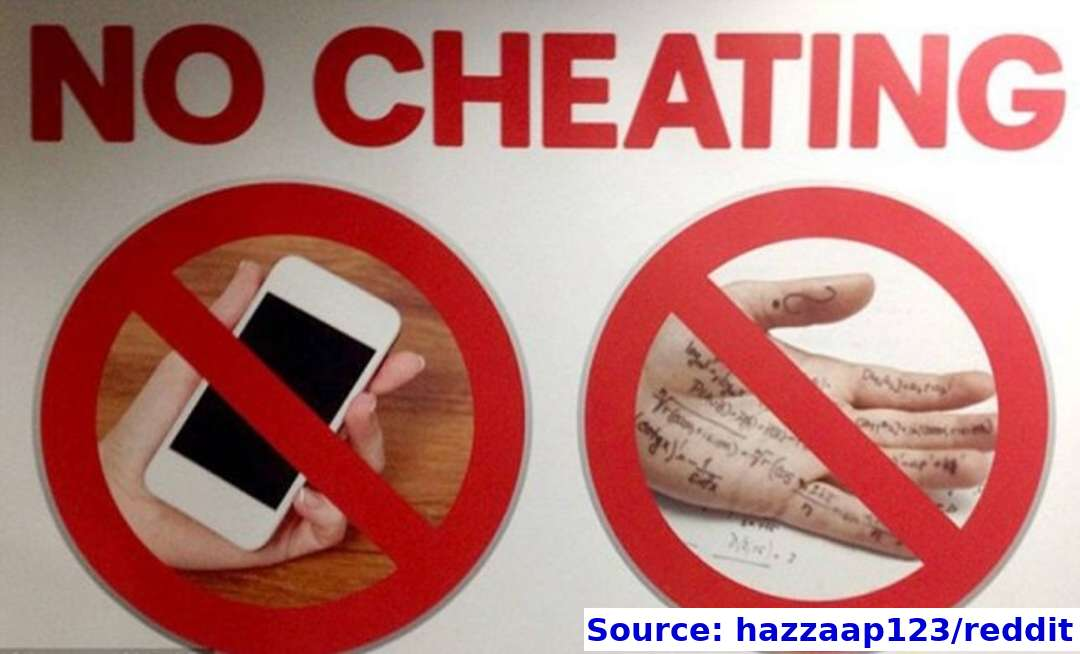
\includegraphics[width=0.37\linewidth]{os-cheating}
\end{figure}

\begin{itemize}
\item All major academic rules violations will be handled directly by the Faculty of Computer Science,
University of Indonesia.
\item ''Accidents'' may happen. There will be warnings for the first two minor violations.
\item Your final grade will be reduced for the third warning.
\item Your final grade will be reduced to "D" for the fourth warning.
\item Five (5) or more warnings will be considered as a significant academic-rules violation.
\end{itemize}

\end{frame}

% XXXXXXXXXXXXXXXXXXXXXXXXXXXXXXXXXXXXXXXXXXXXXXXXXXXXXXXXXXXXXXXXXXXXXXX
\section{Miscellaneous}
\begin{frame}[fragile]
\frametitle{Out of Topic/Intermezzo/Segue}
\begin{itemize}
\item Semiconductor Scalling.
\begin{itemize}
\item 1971: $10 \mu{}m$
\item 1984: $1 \mu{}m$
\item 1996: $250 nm$
\item 2016: $10 nm$
\item 2020: $5 nm$
\item 2022: $3 nm$
\end{itemize}
\item Fairchild Semiconductor Indonesia.
\item National Semiconductor Indonesia.
\item Minister of Manpower (Menteri Tenaga Kerja) 1983–1988.
\item Marvell Technology, Inc (1995).
\item SoC: System on a Chip.
\item SiP: System in a Package.
\item TSMC: Taiwan Semiconductor Manufacturing Company, Ltd.
\item ASML Holding, N.V: Advanced Semiconductor Materials Lithography.
\item Carl Zeiss SMT GmbH (This is NOT Optik Seis, Duh :).
\end{itemize}
\end{frame}

% XXXXXXXXXXXXXXXXXXXXXXXXXXXXXXXXXXXXXXXXXXXXXXXXXXXXXXXXXXXXXXXXXXXXXXX
\begin{frame}[fragile]
\frametitle{The Computing Diciplines}
\begin{figure}
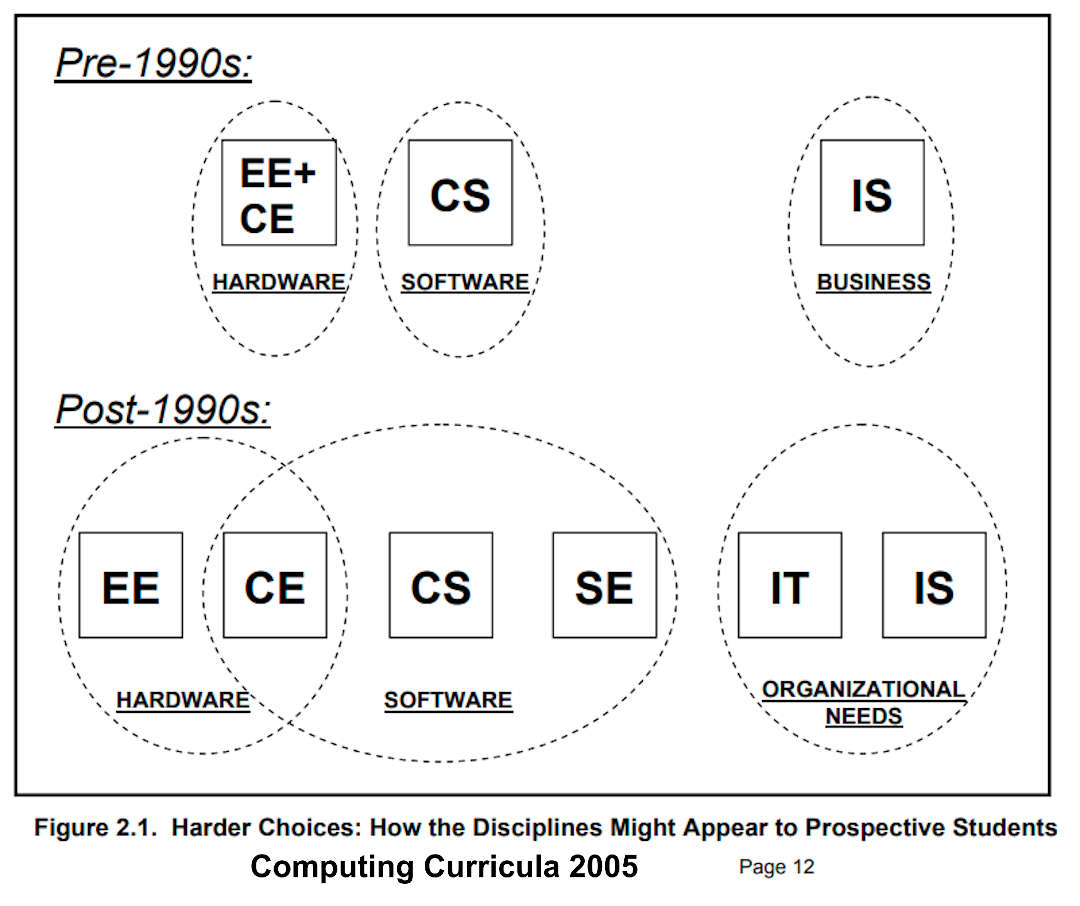
\includegraphics[width=0.59\linewidth]{pic-cc2005}
\caption{The Computing Diciplines}
\end{figure}
\end{frame}

% XXXXXXXXXXXXXXXXXXXXXXXXXXXXXXXXXXXXXXXXXXXXXXXXXXXXXXXXXXXXXXXXXXXXXXXXXX
\section{Assignments}
\begin{frame}[fragile]
\frametitle{Assignments}
\begin{itemize}
\item There will be no mid-term (UTS) nor final-term (UAS).
      Instead, there will be 11 weekly assignments.
      Your grade will be taken from the best 9 out of 11 assignments.
\item You need to run ''VirtualBox'' on a computer with more than 4GB RAM and up to 64 GB disk space.
\item Each assignment deadline will be by the end of that ''week''.
      The weekly schedule will be at \url{https://sp.vlsm.org/\#idx02}.
\item Submit (push) the assignments to \url{https://github.com/}.
      If you still don't have one, you need to sign up for a \url{https://github.com/} account.
      More information will follow.
\item See the assignment list at \url{https://osp4diss.vlsm.org/ASP.html}.
\end{itemize}
\end{frame}

% XXXXXXXXXXXXXXXXXXXXXXXXXXXXXXXXXXXXXXXXXXXXXXXXXXXXXXXXXXXXXXXXXXXXXXXXXX
\section{This is an elective course!}
\begin{frame}[fragile]
\frametitle{This is an elective course!}

\begin{itemize}
\item You are not required to take this course!
\item This course is not for you if you:
\begin{itemize}
\item do not like the Operating Systems course.
\item do not like to get your hands dirty.
\item do not have enthusiasm nor initiative at all.
\item do not like to ''hack''.
\end{itemize}
\item Cold Feet? Second Guess?  You might want to drop this course now (this week)!
\item This is the way!
\end{itemize}

\end{frame}

% XXXXXXXXXXXXXXXXXXXXXXXXXXXXXXXXXXXXXXXXXXXXXXXXXXXXXXXXXXXXXXXXXXXXXXXXXX
\end{document}

